% Source: Code/xband-radar-sim/docs/radar_simulation_technical.tex
% Description: Complete signal flow for a single target at 200m range, 45° azimuth.

\documentclass[border=4pt]{standalone}
\usepackage{algpseudocode}
\usepackage{amsmath,amssymb,amsfonts}
\usepackage[T1]{fontenc}
\usepackage{graphicx}
\usepackage{pgfplots}
\usepackage{tikz}
\usepackage{xcolor}
\pgfplotsset{compat=1.18}
\usetikzlibrary{arrows.meta,positioning,shapes.geometric,calc,patterns,decorations.pathmorphing,3d,angles,quotes}

\definecolor{radargreen}{RGB}{0,255,0}
\definecolor{raycolor}{RGB}{255,165,0}
\definecolor{targetcolor}{RGB}{255,0,0}
\definecolor{groundcolor}{RGB}{139,90,43}
\definecolor{skycolor}{RGB}{135,206,235}
\definecolor{beamcolor}{RGB}{255,255,0}


\begin{document}
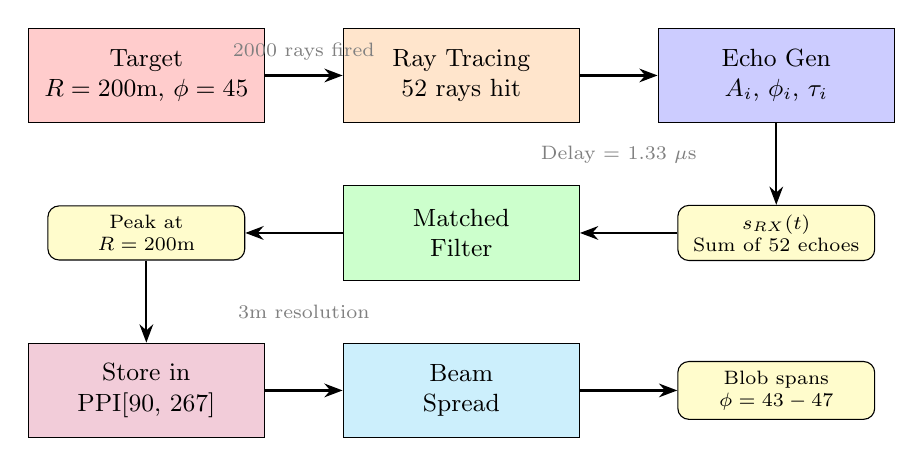
\begin{tikzpicture}[
    box/.style={rectangle, draw, minimum width=3cm, minimum height=1.2cm, align=center, font=\small},
    data/.style={rectangle, rounded corners, draw, fill=yellow!20, minimum width=2.5cm, align=center, font=\scriptsize},
    arrow/.style={-{Stealth}, thick}
]
    % Target info
    \node[box, fill=red!20] (target) at (0,0) {Target\\$R = 200$m, $\phi = 45°$};

    % Ray hits
    \node[box, fill=orange!20] (hits) at (4,0) {Ray Tracing\\52 rays hit};

    % Echo generation
    \node[box, fill=blue!20] (echo) at (8,0) {Echo Gen\\$A_i$, $\phi_i$, $\tau_i$};

    % Received signal
    \node[data] (rx) at (8,-2) {$s_{RX}(t)$\\Sum of 52 echoes};

    % Matched filter
    \node[box, fill=green!20] (mf) at (4,-2) {Matched\\Filter};

    % Compressed
    \node[data] (comp) at (0,-2) {Peak at\\$R = 200$m};

    % Store in PPI
    \node[box, fill=purple!20] (ppi) at (0,-4) {Store in\\PPI[90, 267]};

    % Beam spread
    \node[box, fill=cyan!20] (spread) at (4,-4) {Beam\\Spread};

    % Final
    \node[data] (final) at (8,-4) {Blob spans\\$\phi = 43° - 47°$};

    % Arrows
    \draw[arrow] (target) -- (hits);
    \draw[arrow] (hits) -- (echo);
    \draw[arrow] (echo) -- (rx);
    \draw[arrow] (rx) -- (mf);
    \draw[arrow] (mf) -- (comp);
    \draw[arrow] (comp) -- (ppi);
    \draw[arrow] (ppi) -- (spread);
    \draw[arrow] (spread) -- (final);

    % Annotations
    \node[gray, font=\scriptsize] at (2,0.3) {2000 rays fired};
    \node[gray, font=\scriptsize] at (6,-1) {Delay = 1.33 $\mu$s};
    \node[gray, font=\scriptsize] at (2,-3) {3m resolution};

\end{tikzpicture}
\end{document}
